\documentclass[a4paper, 11pt]{article}
\usepackage{comment} % enables the use of multi-line comments (\ifx \fi) 
\usepackage{lipsum} %This package just generates Lorem Ipsum filler text. 
\usepackage{fullpage} % changes the margin
\usepackage[a4paper, total={7in, 10in}]{geometry}
\usepackage[fleqn]{amsmath}
\usepackage{amssymb,amsthm}  % assumes amsmath package installed
\newtheorem{theorem}{Theorem}
\newtheorem{corollary}{Corollary}
\usepackage{graphicx}
\usepackage{tikz}
\usetikzlibrary{arrows}
\usepackage{verbatim}
%\usepackage[numbered]{mcode}
\usepackage{float}
\usepackage{tikz}
    \usetikzlibrary{shapes,arrows}
    \usetikzlibrary{arrows,calc,positioning}

    \tikzset{
        block/.style = {draw, rectangle,
            minimum height=1cm,
            minimum width=1.5cm},
        input/.style = {coordinate,node distance=1cm},
        output/.style = {coordinate,node distance=4cm},
        arrow/.style={draw, -latex,node distance=2cm},
        pinstyle/.style = {pin edge={latex-, black,node distance=2cm}},
        sum/.style = {draw, circle, node distance=1cm},
    }
\usepackage{xcolor}
\usepackage{mdframed}
%\usepackage[shortlabels]{enumitem}
\usepackage{enumitem}
%\usepackage{indentfirst}
\usepackage{hyperref}
\usepackage{tikz}
\usepackage{csvsimple}
\usepackage{pdflscape}
\usepackage{longtable}

\usetikzlibrary{automata,arrows,positioning,calc}
    
\renewcommand{\thesubsection}{\thesection.\alph{subsection}}

\newenvironment{Exercise}[2][Exercise]
    { \begin{mdframed}[backgroundcolor=gray!20] \textbf{#1 #2} \\}
    {  \end{mdframed}}

% Define solution environment
\newenvironment{solution}
    {\textit{Solution:}}
    {}

\renewcommand{\qed}{\quad\qedsymbol}
%%%%%%%%%%%%%%%%%%%%%%%%%%%%%%%%%%%%%%%%%%%%%%%%%%%%%%%%%%%%%%%%%%%%%%%%%%%%%%%%%%%%%%%%%%%%%%%%%%%%%%%%%%%%%%%%%%%%%%%%%%%%%%%%%%%%%%%%
\begin{document}
%Header-Make sure you update this information!!!!
\noindent
%%%%%%%%%%%%%%%%%%%%%%%%%%%%%%%%%%%%%%%%%%%%%%%%%%%%%%%%%%%%%%%%%%%%%%%%%%%%%%%%%%%%%%%%%%%%%%%%%%%%%%%%%%%%%%%%%%%%%%%%%%%%%%%%%%%%%%%%
\large\textbf{Edward (Ted) Watters} \hfill \textbf{Final Project}   \\
Email: ewatter4@jhu.edu  \\
\normalsize Course: EN.625.722.3VL Probability,Stochastic Process II\\
Term: Spring 2020\\
Professor: Dr. Woolf \\
\noindent\rule{7in}{2.8pt}
\section{Abstract}
Bond credit ratings can be modeled as discrete finite state absorbing Markov chains. Using this, the predictive nature of assigned credit ratings can be compared with the eventual absorbing states of bond default or bond maturity.\\
\\
General findings:
\begin{itemize}
	\item Credit ratings are useful estimators of default likelihood
	\item Default rates associated with credit rating data collected by Mergent tracks with published 3rd party estimates.
	\item There are challenges with data set size, high number of states, and multiple low probability states which cause issues with numerical stability when implementing standard analytical methods. In these cases, simulations are helpful
\end{itemize}

Additionally, bond credit ratings, and their eventual default, maturity, or current state as an active security, occur in predictable sequences. A Hidden Markov Model was used to model these sequences. \\
\\
General findings:
\begin{itemize}
	\item Because of state clumping (e.g. investment grade securities stay investment grade), states repeating themselves, and absorbing states, approximately only 1 hidden state is required for every 2 observed states.
	\item It is likely that a model may fail cross validation because of initial observed states that occur in the test set, but not in the training set. This is because of several observed states having low initial probabilities.
\end{itemize}

All non-proprietary project files are located at: \url{https://github.com/tedwatters/BondCredit}

\section{Data Sources}

Rating History and Default status were exclusively pulled from Wharton's Research Data Services (WRDS) Mergent Fixed Income Security Database (FISD)\cite{wrds}. In particular, data from the Bond Issue and Bond Ratings tables were merged in MySQL. This was a challenge, as the total table has approximately 1.2 million records and over 40 columns. I needed to change my temporary file partition to allow for the up to 80 GB of temporary tables created. Optimizing this MySQL query is future work.\\
\\
WRDS data requires specific access, and the raw files are not located on the project github.\\
\\
This data needed to be filtered and interpreted to be useful for the project. The steps used are available in the github repository. Applicable files include the .sql files, as well as the first portion of the markov model.py file. Specific adjustments included:

\begin{itemize}
	\item Adding a state index value, using the ratings date.
	\item Adding default and maturity states to the time series
	\item Removing duplicate data
	\item Removing errant states
	\item Creating a rule set for how to handle "No Rating" states
	
\end{itemize}

The data set does have some limitations in coverage of securities\cite{wrds-coverage}
\section{Background}

The bond credit system is well described on Wikipedia \cite{wiki_bondcredit}.

\begin{itemize}
	\item There are 3 main credit rating agencies - Fitch, Moody's, and Standard and Poor's
	\item Each credit rating agency has its own nomenclature of ratings, but the general system is similar between agencies.	
\end{itemize}

Consider a simple model of the system with only 2 rating states. A bond is rated by the credit agencies until it either defaults or matures.	
	\begin{center}
		\begin{tikzpicture}[->, >=stealth', auto, semithick, node distance=5cm]
		\tikzstyle{every state}=[fill=white,draw=black,thick,text=black,scale=1]
		\node[state]    (InvestmentGrade)                   {$\text{Investment Grade}$};
		\node[state]    (SpeculativeGrade)[right of=InvestmentGrade]     {$\text{Speculative Grade}$};
		\node[state]    (Default)[below of=SpeculativeGrade]     {$\text{Default}$};
		\node[state]    (Mature)[above of=InvestmentGrade]     {$\text{Mature}$};
		\path
		(InvestmentGrade) edge[loop left]          (InvestmentGrade)
		(SpeculativeGrade) edge[loop right]          (SpeculativeGrade)
		(Default) edge[loop right]          (Default)
		(Mature) edge[loop left]          (Mature);
		\path
		(InvestmentGrade) edge[bend left,below]         (SpeculativeGrade)
		(SpeculativeGrade) edge[bend left,above]         (InvestmentGrade)
		(SpeculativeGrade) edge[bend left,below]         (Default)
		(InvestmentGrade) edge[bend right,above]         (Default)
		(SpeculativeGrade) edge[bend right,above]         (Mature)
		(InvestmentGrade) edge[bend left,above]         (Mature);
		\end{tikzpicture}
	\end{center}

This is a discrete finite state absorbing Markov chain. The step index is simply whenever another rating occurs, which may or many not be at specified time intervals. Rating adjustments can also take place based on events.\\
\\
\begin{landscape}
In practice, we need a separate chain for each rating agency, and each rating agency has a multitude of states within the investment and speculative grades.\\
\\
For example, the transition probability matrix for Fitch is:
	\tiny{\csvautolongtable[
		table head=\caption{Fitch - Transition Probability Matrix $(\mathbf{P})$}\label{tab:some}\\\hline
		\csvlinetotablerow\\\hline
		\endfirsthead\hline
		\csvlinetotablerow\\\hline
		\endhead\hline
		\endfoot,
		respect all
		]{fr_transition_probability_matrix.csv}}
Key observations are:
\begin{itemize}
	\item The absorbing states DEFAULT and MATURE
	\item The likelihood that rating state remains the same between steps is high
	\item There are many near zero values in the matrix. This makes the matrix ill conditioned, so developing numerically stable solutions for certain matrix operations may not be possible. Solutions by simulation may be preferred.	
\end{itemize}
\small
\end{landscape}


\section{Absorption State Analysis}

Discrete finite state absorbing Markov chains have certain properties\cite{absorbing_state}. For instance, the transition probabilty matrix can be broken down into:
$$
\mathbf{P} = \begin{Bmatrix}
	\mathbf{Q} & \mathbf{R} \\
	\mathbf{0} & \mathbf{I}_{s} \\
\end{Bmatrix}
$$
Where $\mathbf{Q}$ is $t \times t$, $\mathbf{R}$ is $t \times s$, and $\mathbf{I}_{s}$ is $s \times s$.\\
\\
Using this, the absorption probability matrix \cite{absorbing_state_wolfram} can be calculated as:
$$  \mathbf{M} = (\mathbf{I}-\mathbf{Q})^{-1} \mathbf{R}$$
Unfortunately, calculating the inverse requires a well conditioned $\mathbf{Q}$. For $(\mathbf{I}-\mathbf{Q})$ associated with the Fitch transition probability matrix, the condition number is 78. Since the log of the condition number is approximately an upper bound for the precision in the matrix \cite{condtion_number}, then the matrix would only be accurate to ~4.4. This is clearly unacceptable for probabilities. Also, when creating an analytical solution, the following matrix was created in Python. This absorption probability matrix uses Gaussian elimination, but similar results were acquired when using numpy's inverse function.\\
	\small{\csvautolongtable[
	table head=\caption{Fitch - Absorption Probability Analytical Solution $(\mathbf{M})$}\label{tab:some}\\\hline
	\csvlinetotablerow\\\hline
	\endfirsthead\hline
	\csvlinetotablerow\\\hline
	\endhead\hline
	\endfoot,
	respect all
	]{fr_absorption_probability.csv}}

When using a simulation to arrive at the absorption probability matrix, results were much more reasonable:
	\small{\csvautolongtable[
	table head=\caption{Fitch - Absorption Probability - Simulation}\label{tab:some}\\\hline
	\csvlinetotablerow\\\hline
	\endfirsthead\hline
	\csvlinetotablerow\\\hline
	\endhead\hline
	\endfoot,
	respect all
	]{fr_absorption_probability_simulation.csv}}
Again, these results are specific to Fitch. However, values for Moody's and Standard and Poor's were similar.\\
\\
These values generally track with historical default rates. However, please note that the data sets that are being used may not be the same (e.g. global vs. US, corporate only vs. corporate + municipal, etc.). Additionally, the absorptive probability that was calculated in the Markov Model measures if the bond \textbf{will ever default} before it matures, given that it is in a certain state now. Figure 1 is specific to a \textbf{1-year period}.

\begin{figure}[h]
	\caption{Standard and Poor's Historical Default Rates\cite{wiki_bondcredit}}
	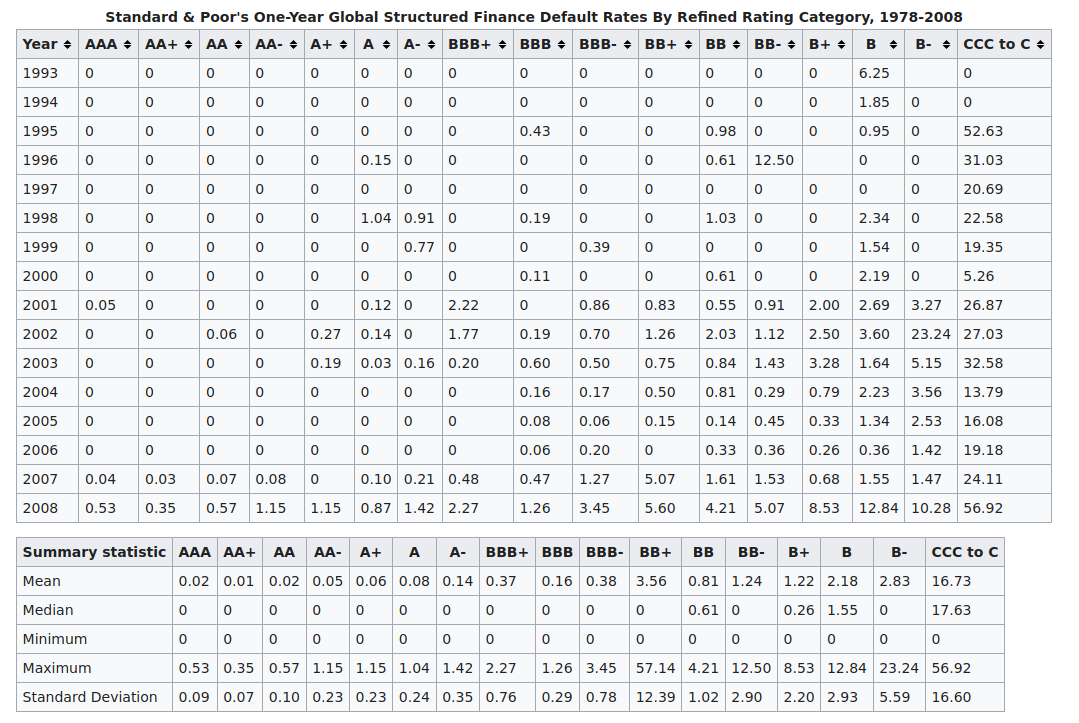
\includegraphics[width=\textwidth]{SPR_Historical_Wikipedia.png}
\end{figure}

\section{Hidden Markov Model (Fitch)}

Because of computing time constraints, I only created a hidden markov model for the Fitch rating data. This included ratings for approximately 150,000 securities.\\
\\
The sequence of observed states used were the ratings states. The sequences are of variable length, depending on if the issue matured, defaulted, or is still active. Additionally, since ratings do not have a fixed periodicity, some securities have more ratings than others.\\
\\
The hidden states are modeled as unknown hyper parameters. To determine the number of hidden states needed, I performed a 5-fold cross validation using between 10 and 15 iterations when fitting for each state.\\
\\
To make the model, I leaned heavily on the Deep Learning Courses Hidden Markov Model in Python online class.\cite{deeplearning-lecture}\cite{deeplearning-github}\\
\\
My hypothesis was that there would be less hidden states than observed states because of data clumping, and the fact that the model is absorptive as $n \longrightarrow \infty$. To test this hypothesis, I randomly split the sequences into 5 groups. I also assigned integer values to each rating state. The code for this is in the hidden markov model python file on the github repository (\url{https://github.com/tedwatters/BondCredit}). There are approximately 32 observed states for each rating agency, so I tested the number of hidden states from 2 to 64. Figure below shows log likelihood of the test set compared to the number of states chosen.

\begin{figure}[!h]
	\caption{Log Likelihood and Number of Hidden States (Fitch data, 5-fold, Test 1, 10 iterations)}
	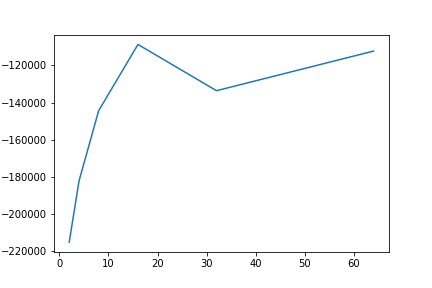
\includegraphics[width=8cm]{M_vs_Likelihood_Test_1.png}
\end{figure}

There was a global maximum at 16 states for this run . It is possible there may be another maximum at >64 states; however, compute time would make a model with this number of states impractical for this project. Based on the state sampling, the optimal number of states is between 9 and 31 (inclusive). Two additional tests were run to look closer at this region. The best estimate of number of hidden states from test 2 was 19 states, which informed values of m tested for the 3rd run, as well as the cross validation. \\
\begin{figure}[!h]
	\caption{Log Likelihood and Number of Hidden States (Fitch data, 5-fold, Test 2, 10 iterations)}
	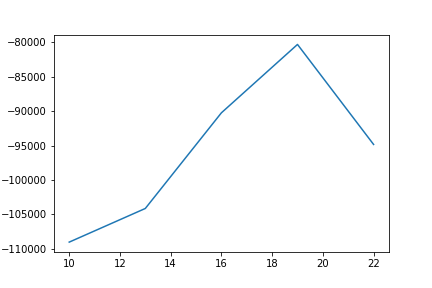
\includegraphics[width=8cm]{M_vs_Likelihood_Test_2.png}
\end{figure}
And tightening the range more tightly around the maximum at 19 hidden states:
\begin{figure}[!h]
	\caption{Log Likelihood and Number of Hidden States (Fitch data, 5-fold, Test 3, 15 iterations)}
	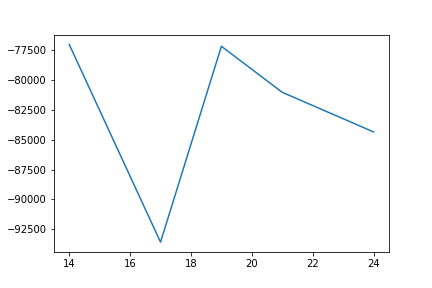
\includegraphics[width=8cm]{M_vs_Likelihood_Test_3.png}
\end{figure}
At this point, I began the process of looking at cross validation. Since partition 0 was used for the initial range investigating, the graph remains the same for this number of hidden states.\\
\\
\begin{figure}[!h]
	\caption{Log Likelihood and Number of Hidden States (Fitch data, 5-fold, Cross validation (Test Set 0), 15 iterations)}
	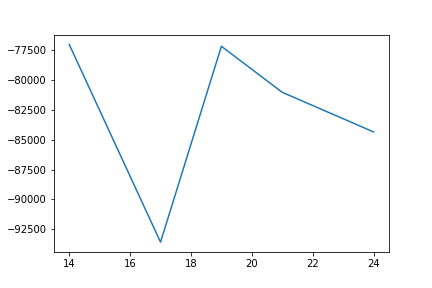
\includegraphics[width=8cm]{Cross_validation_test_0.png}
\end{figure}
Starting with test partition 1, I started to see errors where log likelihood returned at $-\infty$. Specifically, the error was when scaling $\alpha '$ using the equation\cite{deeplearning-scale}:
$$ \hat{\alpha}(t,i) = \frac{\alpha '(t,i)}{c(t)}$$
where:
$$c(t) = \sum_{i=1}^{M}\alpha '(t,i)$$
and:
$$\alpha '(t,i) = \pi_{i}B(j,x(1))$$
The problem was that $c(t)$ was being calculated as 0 for certain partitions, and returning a divide by zero error when calculating. The driver behind this issue is that when initializing the forward-backward algorithm, the following condition must be met:
$$\text{unique initiation states, test set} \subseteq \text{unique initiation states, training set}$$
In this case, only test partitions 1 and 3 met this criteria, thereby causing the scaled forward-backward algorithm to fail. The root cause for this is that are some very rare initial observation states that may get sampled in the test set, but are excluded from the training set.\\
\begin{figure}[!h]
	\caption{Log Likelihood and Number of Hidden States (Fitch data, 5-fold, Cross validation (Test Set 1), 15 iterations)}
	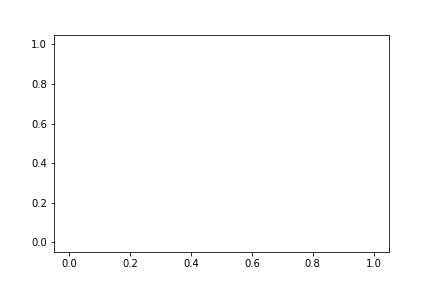
\includegraphics[width=8cm]{Cross_validation_test_1.png}
\end{figure}
\begin{figure}[!h]
	\caption{Log Likelihood and Number of Hidden States (Fitch data, 5-fold, Cross validation (Test Set 2), 15 iterations)}
	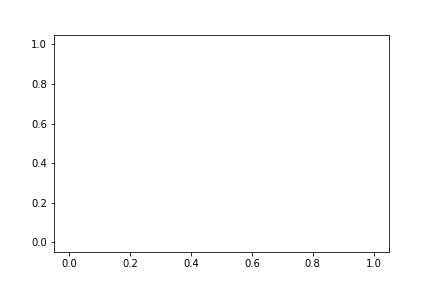
\includegraphics[width=8cm]{Cross_validation_test_2.png}
\end{figure}
\begin{figure}[!h]
	\caption{Log Likelihood and Number of Hidden States (Fitch data, 5-fold, Cross validation (Test Set 3), 15 iterations)}
	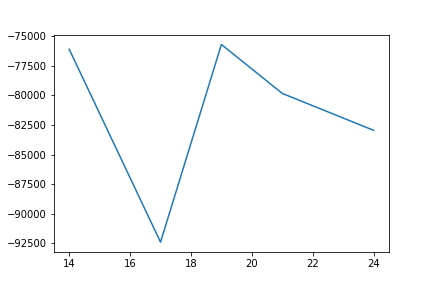
\includegraphics[width=8cm]{Cross_validation_test_3.png}
\end{figure}
\begin{figure}[h]
	\caption{Log Likelihood and Number of Hidden States (Fitch data, 5-fold, Cross validation (Test Set 4), 15 iterations)}
	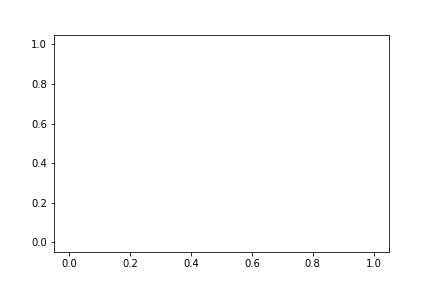
\includegraphics[width=8cm]{Cross_validation_test_4.png}
\end{figure}
\\
Looking at the final  $\mathbf{\pi}$, $\mathbf{A}$, $\mathbf{B}$ generated from test set 4, we can make some generalizations:
\begin{itemize}
	\item $\pi$ -  There are some high (0.581) and low (0.000) initial hidden states. This checks with our understanding that some initial observed states are very common, such as "NR" (0.701), and some almost never occur, such as "DEFAULT". Since the probability of observed state "NR" is higher than the highest probability of the initial hidden states, this suggests that multiple hidden states contribute to initial "NR" ratings. This makes sense because certain sequences such as "NR" $\longrightarrow$ "MATURE" are very common, but so are other "NR" to other rating sequences.
	\item $ \mathbf{A}$ and $ \mathbf{B}$ - In just looking at the Markov chain, it was shown that there is clumping of states. For instance, if a bond was AAA rated before, it will not likely default. It is very likely that it keeps the AAA rating, or goes to another investment grade rating. In the hidden and observed state matrices, The are some very high probabilities in certain rows which indicate state clumping and high predictive power.
\end{itemize}

	\small{\csvautolongtable[
	table head=\caption{Fitch HMM - $\pi$}\label{tab:some}\\\hline
	\csvlinetotablerow\\\hline
	\endfirsthead\hline
	\csvlinetotablerow\\\hline
	\endhead\hline
	\endfoot,
	respect all
	]{hmm_pi.csv}}



	\tiny{\csvautolongtable[
	table head=\caption{Fitch HMM - $\mathbf{A}$}\label{tab:some}\\\hline
	\csvlinetotablerow\\\hline
	\endfirsthead\hline
	\csvlinetotablerow\\\hline
	\endhead\hline
	\endfoot,
	respect all
	]{hmm_A.csv}}

\begin{landscape}
	\tiny{\csvautolongtable[
	table head=\caption{Fitch HMM - $\mathbf{B}$}\label{tab:some}\\\hline
	\csvlinetotablerow\\\hline
	\endfirsthead\hline
	\csvlinetotablerow\\\hline
	\endhead\hline
	\endfoot,
	respect all
	]{hmm_B.csv}}

\end{landscape}

\section{Further Work}

\begin{itemize}\small
	\item Optimize MySQL table merge. Temporary tables took approximately 80GB of hard drive storage during the merge. There may be a more efficient query.
	\item Create Hidden Markov Model based on adjusted data set. Specifically:
	\begin{itemize}
		\item Make steps monthly vs arbitrary rating times (which could be based on initial issue, review based on changes in economic outlook, or just annually)
		\item Add monthly yield data. This would be used as the observed state.
		\item Monthly rating data can be the first known hidden set of states. The hypothesis those bonds with a higher credit rating would have a lower yield.
		\item Create a hyper-parameterized model using just the observed yield data, and an additional model that includes the rating data
		\end{itemize}
	\item Attempt to add additional data sources to validate the WRDS database. Also, attempt to include a larger sphere of fixed income securities.
	\item Utilize cloud computing to:
	\begin{itemize}
		\item Increase the number of iterations run for the hidden markov model during fitting. I ran between 10 and 15 iterations per state in this project. A concern would be that the number of hidden states here is chosen based on quickness of goodness of fit to converge, rather than goodness of fit at convergence.
		\item Increase the number of states tested during cross validation
		\item Increase the number of folds (partitioning into test/ training sets) used during cross validation
		\end{itemize}
	\item Further investigate and generalize the conditions which can lead to failure of a trained hidden markov model to be unable to find the likelihood of a test set.

	
\end{itemize}

\section{Appendix - Raw Data}




	\small{\csvautolongtable[
		table head=\caption{Fitch - Initial State Probability $(\mathbf{\pi})$}\label{tab:some}\\\hline
		\csvlinetotablerow\\\hline
		\endfirsthead\hline
		\csvlinetotablerow\\\hline
		\endhead\hline
		\endfoot,
		respect all
		]{fr_initial_state_probability.csv}}
		
	\small{\csvautolongtable[
		table head=\caption{Moody's - Initial State Probability $(\mathbf{\pi})$}\label{tab:some}\\\hline
		\csvlinetotablerow\\\hline
		\endfirsthead\hline
		\csvlinetotablerow\\\hline
		\endhead\hline
		\endfoot,
		respect all
		]{mr_initial_state_probability.csv}}

	\small{\csvautolongtable[
		table head=\caption{Standard and Poor's - Initial State Probability $(\mathbf{\pi})$}\label{tab:some}\\\hline
		\csvlinetotablerow\\\hline
		\endfirsthead\hline
		\csvlinetotablerow\\\hline
		\endhead\hline
		\endfoot,
		respect all
		]{sprr_initial_state_probability.csv}}


\begin{landscape}		
	\tiny{\csvautolongtable[
		table head=\caption{Fitch - Transition Probability Matrix $(\mathbf{P})$}\label{tab:some}\\\hline
		\csvlinetotablerow\\\hline
		\endfirsthead\hline
		\csvlinetotablerow\\\hline
		\endhead\hline
		\endfoot,
		respect all
		]{fr_transition_probability_matrix.csv}}


\end{landscape}	
\begin{landscape}	
	\tiny{\csvautolongtable[
		table head=\caption{Moody's - Transition Probability Matrix $(\mathbf{P})$}\label{tab:some}\\\hline
		\csvlinetotablerow\\\hline
		\endfirsthead\hline
		\csvlinetotablerow\\\hline
		\endhead\hline
		\endfoot,
		respect all
		]{mr_transition_probability_matrix.csv}}

\end{landscape}	
\begin{landscape}	
	
	\tiny{\csvautolongtable[
		table head=\caption{Moody's - Transition Probability Matrix $(\mathbf{P})$}\label{tab:some}\\\hline
		\csvlinetotablerow\\\hline
		\endfirsthead\hline
		\csvlinetotablerow\\\hline
		\endhead\hline
		\endfoot,
		respect all
		]{spr_transition_probability_matrix.csv}}	
		
\end{landscape}	

	\small{\csvautolongtable[
	table head=\caption{Fitch - Absorption Probability Analytical Solution $(\mathbf{M})$}\label{tab:some}\\\hline
	\csvlinetotablerow\\\hline
	\endfirsthead\hline
	\csvlinetotablerow\\\hline
	\endhead\hline
	\endfoot,
	respect all
	]{fr_absorption_probability.csv}}

	\small{\csvautolongtable[
	table head=\caption{Moody's - Absorption Probability Analytical Solution $(\mathbf{M})$}\label{tab:some}\\\hline
	\csvlinetotablerow\\\hline
	\endfirsthead\hline
	\csvlinetotablerow\\\hline
	\endhead\hline
	\endfoot,
	respect all
	]{mr_absorption_probability.csv}}

	\small{\csvautolongtable[
	table head=\caption{Standard and Poor's - Absorption Probability Analytical Solution $(\mathbf{M})$}\label{tab:some}\\\hline
	\csvlinetotablerow\\\hline
	\endfirsthead\hline
	\csvlinetotablerow\\\hline
	\endhead\hline
	\endfoot,
	respect all
	]{spr_absorption_probability.csv}}	

	\small{\csvautolongtable[
	table head=\caption{Fitch - Absorption Probability - Simulation}\label{tab:some}\\\hline
	\csvlinetotablerow\\\hline
	\endfirsthead\hline
	\csvlinetotablerow\\\hline
	\endhead\hline
	\endfoot,
	respect all
	]{fr_absorption_probability_simulation.csv}}

	\small{\csvautolongtable[
	table head=\caption{Moody's - Absorption Probability - Simulation}\label{tab:some}\\\hline
	\csvlinetotablerow\\\hline
	\endfirsthead\hline
	\csvlinetotablerow\\\hline
	\endhead\hline
	\endfoot,
	respect all
	]{mr_absorption_probability_simulation.csv}}

	\small{\csvautolongtable[
	table head=\caption{Standard and Poor's - Absorption Probability - Simulation}\label{tab:some}\\\hline
	\csvlinetotablerow\\\hline
	\endfirsthead\hline
	\csvlinetotablerow\\\hline
	\endhead\hline
	\endfoot,
	respect all
	]{spr_absorption_probability_simulation.csv}}		

\begin{thebibliography}{9}
	
	\bibitem{wiki_bondcredit}
	Wikipedia - Bond Credit \url{https://en.wikipedia.org/wiki/Bond_credit_rating}
	
	\bibitem{wrds}
	Wharton Research Data Service (WRDS) Mergent Fixed Income Securities Database (FISD) \url{https://wrds-web.wharton.upenn.edu/wrds/ds/fisd/index.cfm}
	
	\bibitem{wrds-coverage}
	Wharton Research Data Service (WRDS) Mergent Fixed Income Securities Database (FISD) Items Not in Coverage \url{https://wrds-www.wharton.upenn.edu/documents/740/Not_Part_of_FISD_Coverage.pdf}	
	
	\bibitem{absorbing_state}
	Brilliant.org - Absorbing Markov Chains \url{https://brilliant.org/wiki/absorbing-markov-chains/}

	\bibitem{absorbing_state_wolfram}
	Wolfram - Absorbing Markov Chains \url{https://demonstrations.wolfram.com/AbsorbingMarkovChain/}	
	
	\bibitem{condtion_number}
	Wolfram - Condition Number \url{https://mathworld.wolfram.com/ConditionNumber.html}	
	
	\bibitem{deeplearning-lecture}
	Deep Learning Courses - Lecture on Discrete HMM Code \url{https://deeplearningcourses.com/lectures/10504}	
	
	\bibitem{deeplearning-github}
	Deep Learning Courses - Lecture on Discrete HMM Code \url{https://github.com/lazyprogrammer/machine_learning_examples/tree/master/hmm_class}	
	
	\bibitem{deeplearning-scale}
	Deep Learning Courses - Lecture on Underflow and Scaling \url{https://deeplearningcourses.com/lectures/10505}		
\end{thebibliography}	

\noindent\rule{7in}{2.8pt}
\end{document}